\chapter{Detekcia farby}

V predchádzajúcej kapitole sme opísali ako vyzerá náš dataset ako sme ho vytvorili.
Táto kapitola je venovaná nášmu prvému modelu neurónovej siete.
Ešte pred vytvorením zložitých a výpočtovo náročných algoritmov, určených na vizualizáciu hudby, bolo nevyhnutné dokázať, že naše dáta nesú informáciu, ktorá dovoľuje takýto počin.

Najjednoduchšia forma vizualizácie hudobnej skladby je reprezentácia farbou.
Pri počúvaní hudby si ľudský mozog dokáže predstaviť obraz.
Tento obraz nemusí obsahovať konkrétne objekty, ale môže byť čisto abstraktný s veľkou dominanciou farby.
Náš algoritmus by mal dokázať podobnú vec.

\section{Návrh}
Na klasifikáciu sme využili neurónovú sieť s troma skrytými vrstvami a jednou výstupnou vrstvou.
Pričom sa každá skrytá vrstva skladá zo sto neurónov.
Na vstupe očakávame dáta na 549 kanáloch.
Výstupom je vektor \(y\) s pätnástimi dimenziami.
Veľkosť tohto vektora súvisí s využitím techniky One-Hot-Encoding.
Zo vstupných dát model určuje jednu z pätnástich farieb, preto je pre každú farbu priradený jeden rozmer.
Aktivačnou funkciou pre jednotlivé vrstvy je ReLu (obrázok \ref{relu}).
\begin{figure}[!ht]
	\centering
	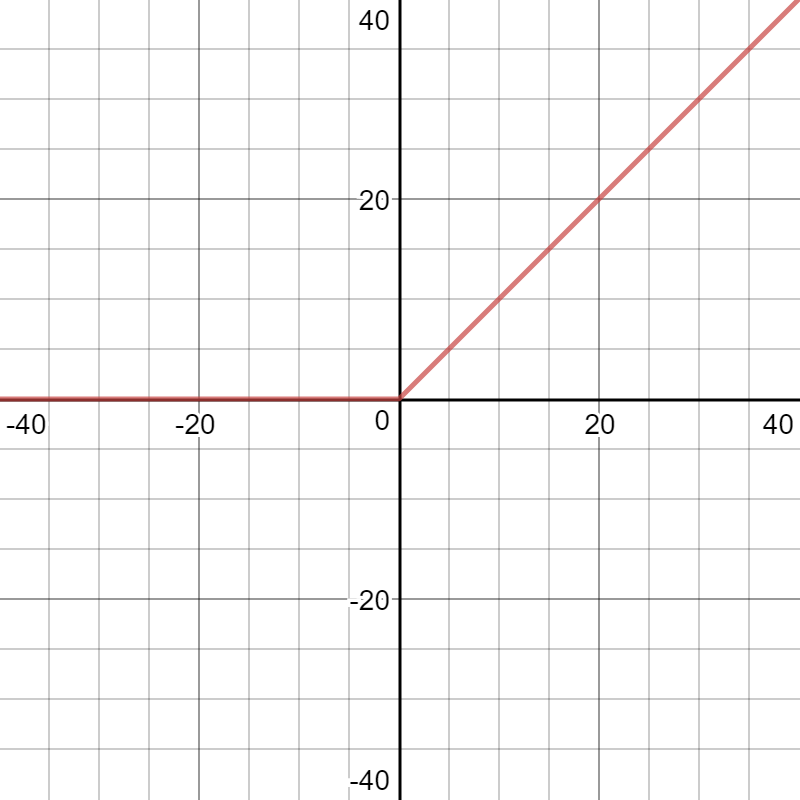
\includegraphics[width=.4\textwidth]{figures/relu}
	\caption{Graf aktivačnej funkcie ReLu.}
	\label{relu}
\end{figure}
ReLu je definovaná ako \[g(x) = max(0, x)\]
Pričom obor hodnôt je \(H = <0, \infty)\).

Trénovanie modelu je realizované v troch krokoch.
Výpočty sú vykonávané na dávkach dát.
V prvom kroku je vytvorená predikcia výsledku.
Následne sú tieto výsledky porovnané s očakávanými výstupmi a vypočíta sa chyba.
Táto chyba je vstupom do optimalizátoru, ktorý upraví premenné siete.
Celý proces sa opakuje vo viacerých epochách pre dosiahnutie väčšej presnosti.

Na výpočet rozdielu medzi výstupom neurónovej siete a predpokladaným výstupom využijeme krížovú entropiu.
Krížová entropia pre dve diskrétne rozdelenia pravdepodobností \(p\) a \(q\) je definovaná ako \[H(p,q) = - \sum p(x)\log q(x)\]

Optimalizovanie premenných modelu, čiže váhových matíc a prahov excitácie zabezpečí algoritmus spätného šírenia chyby.
Konkrétne ide o modifikáciu algoritmu Gradient Descent.

\section{Implementácia}
Model klasifikátora a jeho trénovanie je implementované v jazyku python, využitím modulu TensorFlow.
TensorFlow obsahuje mnoho algoritmov strojového učenia, preto nás oslobodzuje od ich implementovania.
Ďalšou výhodou tohto modulu je to, že separuje výpočty od pythonu, preto sú tieto výpočty rýchlejšie a je možné ich paralelizovať.
Program pozostáva z dvoch krokov, vytvorenie výpočtového grafu a jeho spustenie.
Výpočtový graf obsahuje celý model neurónovej siete spolu so všetkými výpočtovými krokmi pre trénovanie.

Vďaka tomu je možné implementovať funkciu pre trénovanie len niekoľkými riadkami.
\begin{minted}{python}
with tf.Session() as sess:
	sess.run(tf.global_variables_initializer())
	for epoch in range(hm_epochs):
		for _ in range(num_examples/batch_size):
			epoch_x, epoch_y = next_batch(batch_size)
			sess.run([optimizer, cost], 
				feed_dict={x: epoch_x, y: epoch_y})
\end{minted}

Na začiatku je nutné nainicializovať premenné, až potom je možné s nimi pracovať.
V každej epoche sú prejdené všetky dáta a sú optimalizované premenné siete.
Výpočty sa spúšťajú príkazom run.
Jeho parametrami sú výpočty, vrcholy TensorFlow grafu, a vstupné premenné potrebné pre tieto výpočty.
Optimizer je verzia algoritmu Gradient Descent.
\begin{minted}{python}
optimizer = tf.train.AdamOptimizer().minimize(cost)
\end{minted}
Na výpočet chyby (cost) je využitá TensorFlow implementácia krížovej entropie.
\begin{minted}{python}
prediction = neural_network_model(x)
cost = tf.reduce_mean(tf.nn.softmax_cross_entropy_with_logits(
			logits=prediction, 
			labels=y))
\end{minted}
